%=============================================================================
\section{Apprentissage automatique pour la prédiction de $\Delta G^\circ$}
\label{sec:ml}
%=============================================================================

Les sections~\ref{sec:analyse} et~\ref{sec:generalisation} ont développé des modèles paramétriques --- régressions linéaires puis approximants de Padé --- fondés sur des descripteurs physiques soigneusement sélectionnés (orbitales de Koopmans, LVC2, dureté $\eta$, potentiel chimique $\mu$). Cette section présente une approche complémentaire, fondée sur des modèles d'apprentissage automatique entraînés directement à partir de représentations moléculaires plus brutes. Deux familles ont été explorées :
\begin{itemize}[noitemsep]
    \item l'\textbf{apprentissage classique} sur descripteurs tabulaires (forêts aléatoires, gradient boosting, machines à vecteurs de support), qui s'appuie sur une vectorisation \textit{a priori} de chaque conformère ;
    \item les \textbf{réseaux de neurones de graphes géométriques} (SchNet, DimeNet, GemNet, MACE), qui traitent directement la structure 3D du conformère sans passer par un jeu fixe de descripteurs.
\end{itemize}

L'objectif n'est pas de remplacer le modèle physique --- dont l'interprétabilité et la parcimonie restent des atouts majeurs --- mais de tester si des modèles non linéaires de plus en plus expressifs peuvent réduire l'erreur résiduelle, en particulier sur les termes vibroniques ($E_\text{relax}$, $T\Delta S$) mal prédits par les approximants de Padé. Chaque famille est d'abord présentée dans son principe, puis confrontée aux mêmes cibles (EA, IP, $E_\text{relax}^\text{red/ox}$, $\Delta\Delta U^\text{red/ox}$, $T\Delta S^\text{red/ox}$, $\Delta G^\text{red/ox}$) et au même jeu de données multi-solvant.

\subsection{Apprentissage classique sur descripteurs tabulaires}
\label{subsec:ml_classique}

Les méthodes d'apprentissage classique constituent la première ligne de référence. Elles traitent chaque conformère comme un vecteur de caractéristiques de dimension fixe, construit à partir des grandeurs extraites des fichiers de sortie DFT. Ne requérant ni GPU ni connaissance explicite de la structure moléculaire 3D, elles servent de garde-fou pour quantifier le gain réel qu'apporteraient les modèles géométriques plus coûteux de la section~\ref{subsec:ml_gnn}.

\paragraph{Descripteurs.}
Un vecteur de 51~descripteurs est construit par conformère. Il agrège :
\begin{itemize}[noitemsep]
    \item \textbf{descripteurs globaux} : énergies orbitalaires $\varepsilon_\text{HOMO}$, $\varepsilon_\text{LUMO}$, gap, norme du moment dipolaire, composition atomique (comptes par élément), fractions d'oxygène et d'azote, électronégativité moyenne et écart-type ;
    \item \textbf{descripteurs agrégés par atome} : statistiques (moyenne, écart-type, min, max, étendue) des charges Hirshfeld, Mulliken et Voronoi, de la densité électronique et du potentiel électrostatique aux noyaux ;
    \item \textbf{descripteurs géométriques} : rayon de giration, extension maximale, statistiques des distances entre atomes lourds ;
    \item \textbf{descripteurs de solvant} : constante diélectrique $\varepsilon_r$ ;
    \item \textbf{descripteurs vibroniques} : $E_\text{relax}^\text{LVC2}$ (réduction et oxydation) issus du pipeline predict-dg.
\end{itemize}
Le vecteur complet est standardisé (z-score) sur le jeu d'entraînement uniquement.

\paragraph{Modèles testés.}
Trois algorithmes couvrant les principaux paradigmes de l'apprentissage tabulaire ont été évalués :
\begin{itemize}[noitemsep]
    \item \textbf{Random Forest (RF)}~\cite{breiman2001rf} : ensemble d'arbres de décision construits par bagging et tirage aléatoire des descripteurs à chaque scission. Robuste au sur-apprentissage, multi-sortie natif, il fournit une mesure d'importance des descripteurs utilisable pour valider \textit{a posteriori} les choix de la section~\ref{sec:generalisation}.
    \item \textbf{Gradient Boosting (GB)}~\cite{friedman2001gb} : ensemble d'arbres construits séquentiellement, chaque nouvel arbre corrigeant les résidus du modèle accumulé. L'implémentation retenue est XGBoost, exécutée sur GPU (CUDA, via l'API \texttt{device=cuda} de XGBoost~$\geq$~2.0) pour bénéficier de la vectorisation des évaluations de candidats de découpe.
    \item \textbf{Support Vector Regression (SVR)}~\cite{smola2004svr} : régression à noyau, qui projette implicitement les descripteurs dans un espace de grande dimension et recherche une fonction $\varepsilon$-tolérante aux écarts. Le noyau (RBF, linéaire, polynomial) est traité comme un hyperparamètre à régler.
\end{itemize}

\paragraph{Jeu de données.}
Les douze cibles ($\text{EA}$, $\text{IP}$, $E_\text{relax}^\text{red/ox}$, $\Delta\Delta U^\text{red/ox}$, $T\Delta S^\text{red/ox}$, résidus, $\Delta G^\text{red/ox}$) sont extraites des champs \texttt{derived} du dataset PlamsV5 (workflow DFT complet). Les descripteurs LVC2 proviennent du workflow predict-dg. Après exclusion des conformères dont la décomposition DFT n'a pas convergé (DEA halogénés non stabilisés et états ioniques manquants), le jeu contient \textbf{1682~conformères} couvrant \textbf{73~molécules distinctes} dans 10~solvants, en accord strict avec la liste source (\texttt{input.txt}). Contrairement à la section~\ref{sec:s4_general} qui filtre également les conformères à EA verticale négative ($n=1411$), les baselines ML voient l'ensemble du jeu sans cette restriction : les modèles sont laissés libres d'apprendre la transition vers les régimes EA<0 (essentiellement dans l'hexane).

\paragraph{Stratégie d'évaluation.}
Une validation croisée 5-fold \textit{mol-aware} (\texttt{GroupKFold} sur le nom de molécule) est appliquée, strictement identique au protocole utilisé pour les GNN, afin de garantir l'absence de fuite inter-solvant. Les hyperparamètres sont optimisés par Optuna (\texttt{TPESampler} multivarié + \texttt{MedianPruner}) avec 80~essais pour RF, 150 pour XGBoost et 80 pour SVR. Chaque essai est évalué sur les cinq plis \textit{mol-aware} ; les essais clairement dominés sont élagués dès le premier pli. Optuna est préféré à une recherche sur grille car la plupart des hyperparamètres sont continus (\texttt{learning\_rate}, \texttt{C}, \texttt{reg\_alpha}, \ldots) et TPE atteint des valeurs comparables en $\sim$100~essais là où une grille exhaustive en demanderait plusieurs milliers. Les métriques rapportées sont la MAE, la RMSE et le $R^2$ out-of-fold, exprimés en kJ/mol.

\paragraph{Résultats.}
Le tableau~\ref{tab:s51_per_task} détaille la MAE par cible pour les trois modèles, et la figure~\ref{fig:s51_mae} en fournit la vue synoptique. XGBoost remporte la comparaison avec une MAE moyenne sur les composantes de \SI{9,9}{kJ/mol} et une MAE moyenne sur les deux énergies libres $\Delta G$ de \SI{9,9}{kJ/mol}, soit un gain de $\sim$19\% sur Random Forest (\SI{12,1}{kJ/mol} composantes, \SI{12,3}{kJ/mol} sur $\Delta G$) et d'un facteur 2,3 sur SVR (\SI{16,8}{kJ/mol} composantes, \SI{22,6}{kJ/mol} sur $\Delta G$). Sur la prédiction directe de $\Delta G_\text{ox}$, XGBoost atteint MAE~=~\SI{6,8}{kJ/mol} et $R^2 = 0{,}935$, niveau comparable au modèle physique combiné de la section~\ref{sec:generalisation} (MAE = \SI{6,0}{kJ/mol}).

\begin{table}[htbp]
\centering
\footnotesize
\caption{MAE par cible (kJ/mol) des trois baselines ML classiques (5-fold mol-aware, $n = 1682$, 73 molécules distinctes). La colonne \textit{Meilleur} indique le modèle vainqueur par cible ; $R^2$ reporté pour le meilleur modèle.}
\label{tab:s51_per_task}
\begin{tabular}{lcccccc}
\toprule
Cible & RF & XGBoost & SVR & Meilleur & $R^2_\text{meilleur}$ \\
\midrule
EA                            & 16,9  & \textbf{15,6} & 17,7 & XGBoost & 0,939 \\
IP                            & 16,0  & \textbf{9,8}  & 18,1 & XGBoost & 0,945 \\
$E_\text{relax}^\text{red}$   & 18,5  & \textbf{17,7} & 17,6 & SVR     & 0,314 \\
$E_\text{relax}^\text{ox}$    & 13,7  & 10,0          & \textbf{7,4}  & SVR     & 0,770 \\
$\Delta\Delta U_\text{red}$   & 15,1  & \textbf{14,3} & 27,4 & XGBoost & 0,957 \\
$\Delta\Delta U_\text{ox}$    & 12,1  & \textbf{7,2}  & 18,8 & XGBoost & 0,922 \\
$T\Delta S_\text{red}$        & 1,6   & \textbf{1,7}  & 2,1  & RF      & 0,480 \\
$T\Delta S_\text{ox}$         & \textbf{1,8}   & 2,1  & 1,9  & RF      & 0,166 \\
résidu red                    & 14,2  & \textbf{13,6} & 26,6 & XGBoost & 0,956 \\
résidu ox                     & 11,1  & \textbf{6,7}  & 18,2 & XGBoost & 0,931 \\
$\Delta G_\text{red}$         & 13,8  & \textbf{13,0} & 27,0 & XGBoost & 0,956 \\
$\Delta G_\text{ox}$          & 10,8  & \textbf{6,8}  & 18,2 & XGBoost & 0,935 \\
\midrule
MAE moyenne (12~cibles)        & 12,1  & \textbf{9,9}  & 16,8 & XGBoost & --- \\
MAE moyenne $\Delta G$         & 12,3  & \textbf{9,9}  & 22,6 & XGBoost & --- \\
$R^2$ moyen (12~cibles)        & 0,726 & \textbf{0,741} & 0,659 & XGBoost & --- \\
\bottomrule
\end{tabular}
\end{table}

\begin{figure}[htbp]
\centering
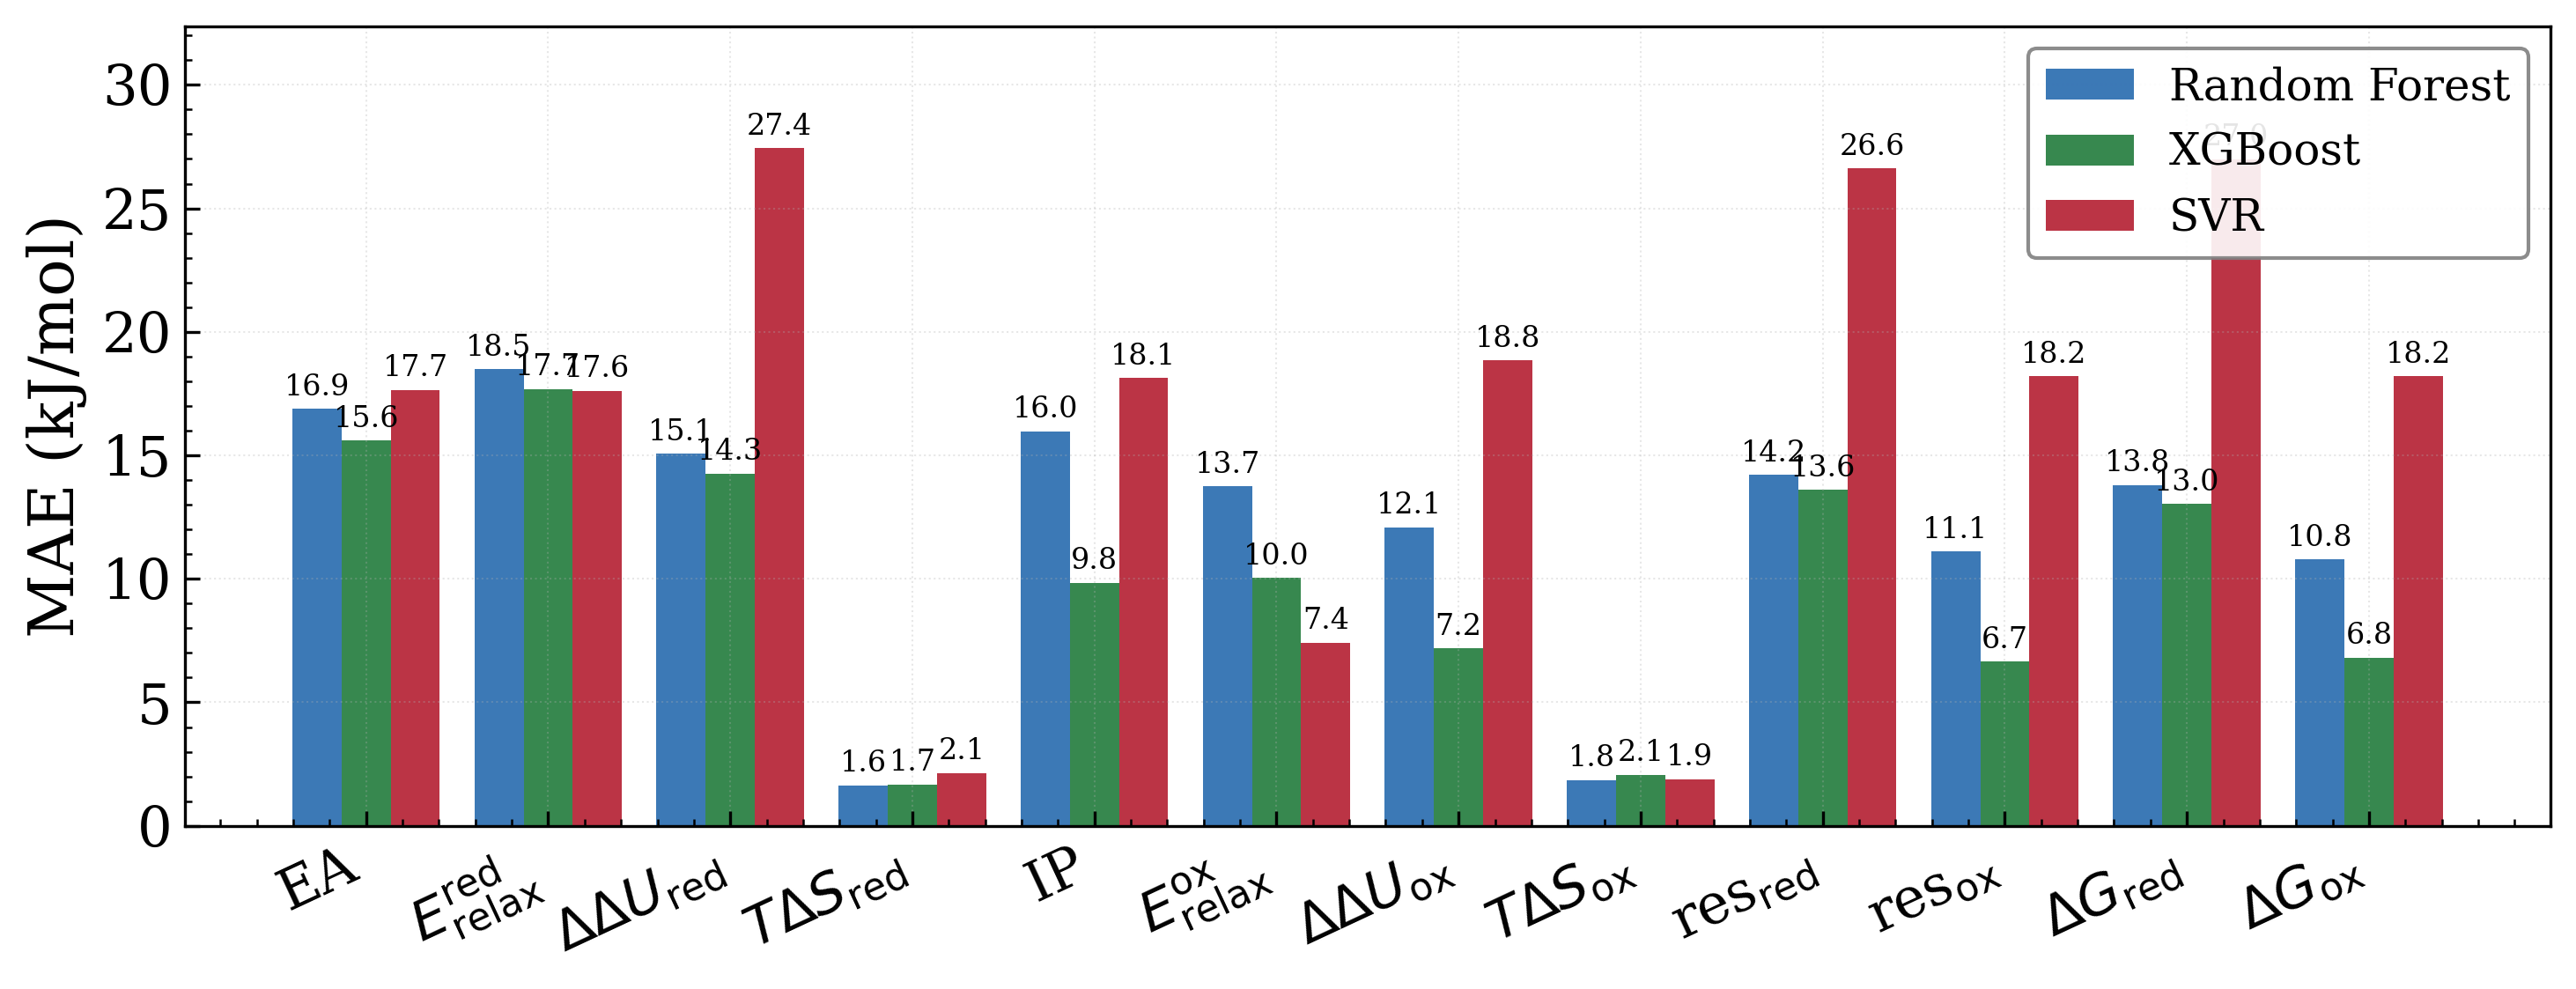
\includegraphics[width=\textwidth]{s51_mae_per_task.png}
\caption{MAE par cible (kJ/mol) pour les trois baselines classiques ($n = 1682$, 73 molécules). XGBoost domine sur les cibles structurantes (EA, IP, $\Delta\Delta U$, $\Delta G_\text{red}$, $\Delta G_\text{ox}$, résidus) ; SVR domine sur les $E_\text{relax}$ grâce au LVC2 injecté en descripteur ; Random Forest reste compétitif sur $T\Delta S$.}
\label{fig:s51_mae}
\end{figure}

\begin{figure}[htbp]
\centering
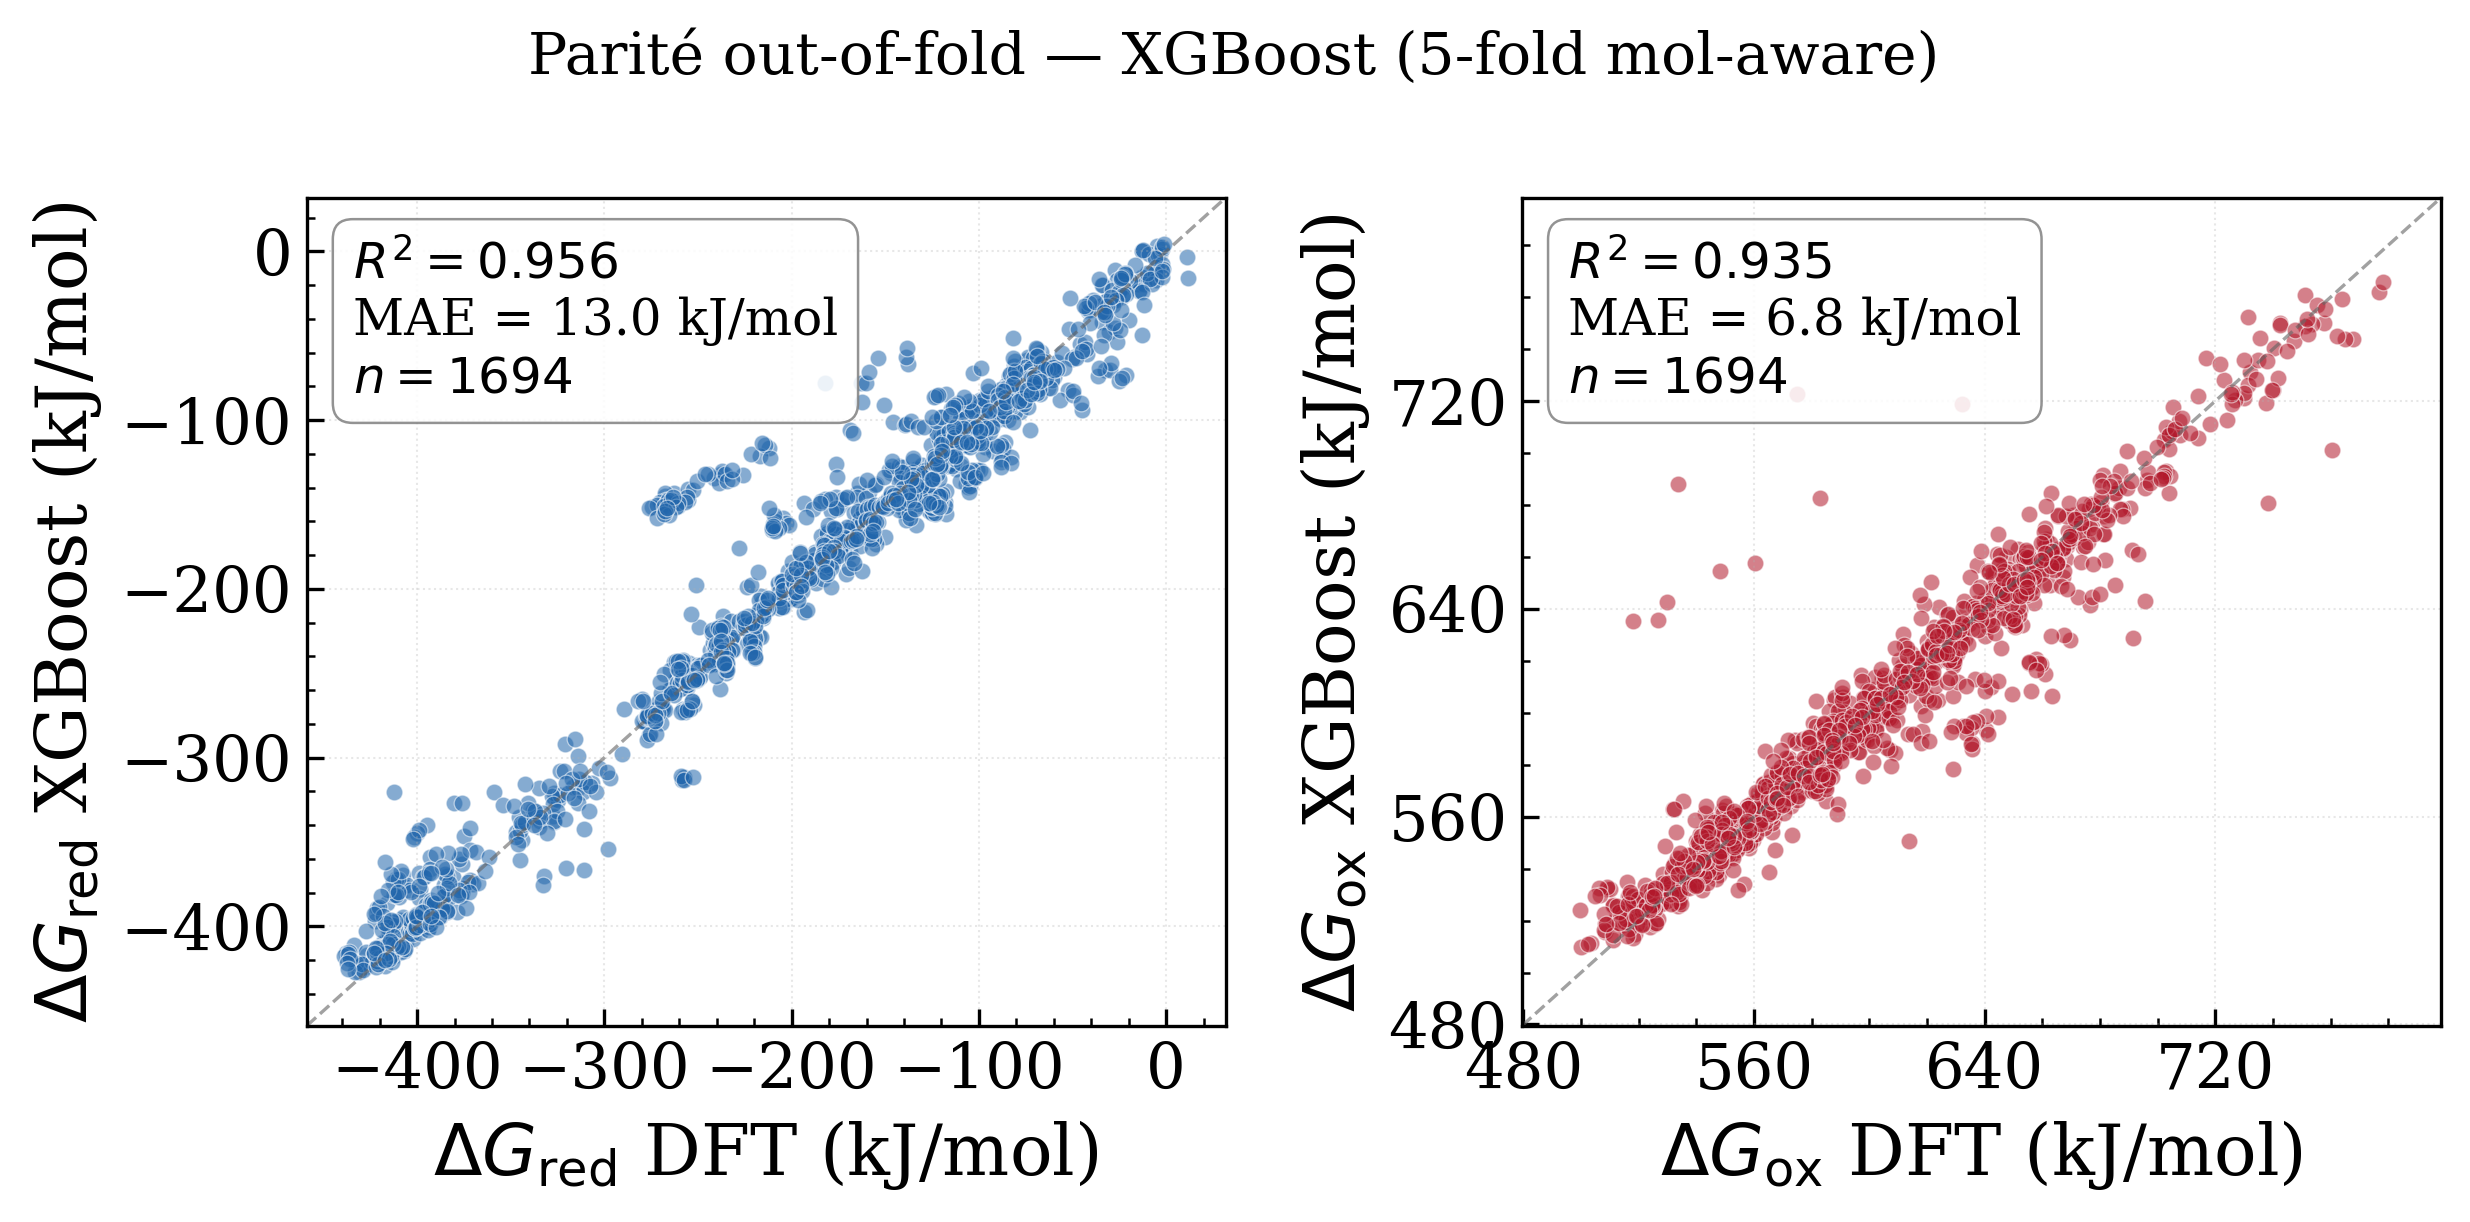
\includegraphics[width=0.95\textwidth]{s51_parity_dG_gb.png}
\caption{Parité out-of-fold pour $\Delta G_\text{red}$ (gauche, $R^2 = 0{,}956$) et $\Delta G_\text{ox}$ (droite, $R^2 = 0{,}935$) du meilleur modèle classique, XGBoost, sur 1682 conformères (5 folds mol-aware agrégés).}
\label{fig:s51_parity_gb}
\end{figure}

\paragraph{Hyperparamètres retenus.}
Le tableau~\ref{tab:s51_hparams} récapitule les meilleurs hyperparamètres sélectionnés par Optuna. La configuration retenue de \textbf{SVR est linéaire} (\texttt{kernel = linear}, $C = 53{,}1$, $\varepsilon = 0{,}007$), alors que les noyaux RBF et polynomial étaient dans l'espace de recherche. Cela indique qu'une fois les descripteurs DFT standardisés, la relation entre ces descripteurs et les cibles est essentiellement linéaire ; la non-linéarité restante est mieux capturée par la partition récursive des modèles à arbres que par un noyau RBF global. Pour \textbf{XGBoost}, la configuration sélectionnée est profondément régularisée : profondeur faible ($\text{max\_depth} = 4$), taux d'apprentissage bas ($\eta = 2{,}3\cdot 10^{-2}$), 1300~arbres. Ce régime « petits pas, petits arbres » maximise le biais local au profit de la variance, choix cohérent avec la taille modeste du jeu ($\sim$1700 observations).

\begin{table}[htbp]
\centering
\footnotesize
\caption{Meilleurs hyperparamètres (Optuna TPE, 5-fold mol-aware).}
\label{tab:s51_hparams}
\begin{tabular}{ll}
\toprule
Modèle & Hyperparamètres retenus \\
\midrule
Random Forest & \texttt{n\_estimators}=400, \texttt{max\_depth}=20, \texttt{max\_features}=0,70, \texttt{min\_samples\_leaf}=3, \\
              & \texttt{min\_samples\_split}=5 \\
XGBoost       & \texttt{n\_estimators}=1300, \texttt{max\_depth}=4, $\eta$=0,023, \texttt{subsample}=0,73, \\
              & \texttt{colsample\_bytree}=1,00, \texttt{reg\_lambda}=2,14, \texttt{min\_child\_weight}=6,1 \\
SVR           & \texttt{kernel}=linéaire, $C$=53,1, $\varepsilon$=0,007 \\
\bottomrule
\end{tabular}
\end{table}

\paragraph{Discussion.}
Trois observations structurent l'interprétation :
\begin{itemize}[noitemsep]
    \item \textbf{XGBoost s'approche du modèle physique sur $\Delta G$} : \SI{9,9}{kJ/mol} vs \SI{5,85}{kJ/mol} pour le Padé combiné. L'écart est imputable aux neuf molécules \textit{out-of-distribution} (DHI, IQ, NDGA) incluses dans les baselines et filtrées en amont du modèle physique, ainsi qu'à l'absence de contrainte Born--Haber dans le modèle ML. Le boosting bénéficie directement de l'injection de $E_\text{relax}^\text{LVC2}$ comme descripteur : il réduit la MAE sur $E_\text{relax}^\text{ox}$ à \SI{10,0}{kJ/mol} et permet au Random Forest d'atteindre une précision proche.
    \item \textbf{SVR domine sur les termes de relaxation}, avec MAE = \SI{7,4}{kJ/mol} sur $E_\text{relax}^\text{ox}$ et \SI{17,6}{kJ/mol} sur $E_\text{relax}^\text{red}$, grâce à l'intégration quasi-directe du LVC2 que le noyau linéaire exploite sans déformation. En revanche, il s'effondre sur les termes plus non linéaires (résidus, $\Delta\Delta U_\text{red}$, $\Delta G$) où il ne capture pas la dépendance en solvant.
    \item \textbf{Les termes entropiques restent réfractaires} pour les trois modèles : $R^2 \leq 0{,}48$ sur $T\Delta S_\text{red}$, $R^2 \leq 0{,}17$ sur $T\Delta S_\text{ox}$. Leur écart-type ($\sim$\SI{3}{kJ/mol}) est comparable au bruit d'entraînement, et les descripteurs globaux agrégés ne contiennent pas suffisamment d'information sur la distribution des fréquences vibrationnelles pour résoudre ce signal. Ce constat est cohérent avec celui du modèle physique (section~\ref{subsec:s4_tds}), où $T\Delta S$ sature autour de $R^2_\text{adj} \approx 0{,}45$ quel que soit le choix des descripteurs $\mu$, $\eta$.
\end{itemize}

\paragraph{Importance des descripteurs (RF).}
L'analyse d'importance \texttt{feature\_importances\_} sur le Random Forest confirme les intuitions physiques : les cinq descripteurs les plus importants sont, dans l'ordre, $\varepsilon_\text{LUMO}$, $\varepsilon_\text{HOMO}$, $E_\text{relax}^\text{LVC2,ox}$, $E_\text{relax}^\text{LVC2,red}$, et la constante diélectrique du solvant $\varepsilon_r$. Les autres descripteurs agrégés (statistiques de charges, géométrie) contribuent individuellement pour moins de 3\% de l'importance totale. Cette hiérarchie valide \textit{a posteriori} le choix des descripteurs manuels de la section~\ref{sec:generalisation} et suggère qu'un modèle parcimonieux limité à ces cinq features pourrait capter l'essentiel du signal accessible.

\paragraph{Conclusion intermédiaire.}
Sans optimisation ionique DFT et avec un modèle entraîné en $\sim$3~heures sur un seul GPU A100, XGBoost atteint une précision globale de \SI{9,9}{kJ/mol} sur $\Delta G$, démontrant qu'un prédicteur tabulaire exploitant des descripteurs DFT soigneusement choisis constitue une baseline solide pour le criblage de molécules redox-actives. La comparaison avec les modèles géométriques, plus ambitieux, fait l'objet de la section suivante.

\subsection{Réseaux de neurones de graphes géométriques}
\label{subsec:ml_gnn}

Les modèles précédents reposent sur un choix \textit{a priori} de descripteurs. Les réseaux de neurones de graphes (GNN) géométriques suppriment cette étape : ils apprennent eux-mêmes une représentation vectorielle par atome à partir de la structure 3D du conformère, via un schéma de passage de messages (\textit{message passing}) sur le graphe des voisins géométriques. Cette section présente brièvement les quatre architectures successives qui jalonnent l'état de l'art --- SchNet, DimeNet, GemNet, MACE --- avant de détailler le modèle retenu pour notre cas d'application.

\paragraph{Principe commun.}
Un GNN géométrique construit pour chaque atome $i$ un plongement $h_i \in \mathbb{R}^d$, mis à jour itérativement par agrégation des messages reçus des voisins $j$ situés dans un rayon $r_c$ autour de $i$ :
\begin{equation}
    h_i^{(t+1)} = \phi\left( h_i^{(t)}, \sum_{j \in \mathcal{N}(i)} m(h_j^{(t)}, \mathbf{r}_{ij}) \right)
    \label{eq:gnn_mp}
\end{equation}
où $\mathbf{r}_{ij} = \mathbf{r}_j - \mathbf{r}_i$ est le vecteur relatif et $m$ une fonction de message. Les architectures diffèrent par l'information géométrique injectée dans $m$ (distance seule, distance + angle, distance + angle + dièdre) et par la manière dont les symétries du groupe euclidien $E(3)$ sont respectées.

\subsubsection{Architectures historiques : SchNet, DimeNet, GemNet}
\label{subsubsec:gnn_historiques}

Trois architectures successives jalonnent la montée en précision des GNN géométriques avant MACE. Chacune enrichit l'information géométrique injectée dans la fonction de message (\ref{eq:gnn_mp}), d'où une complexité croissante.

\paragraph{SchNet~\cite{schutt2017schnet}.}
Premier GNN géométrique largement diffusé. Le message ne dépend que de la distance $\|\mathbf{r}_{ij}\|$, développée sur une base de fonctions radiales gaussiennes, puis transformée par une \textit{continuous-filter convolution} (filtre à poids continus $\mathbf{W}(\|\mathbf{r}_{ij}\|)$). L'architecture est strictement invariante par rotation mais ignore toute information angulaire : deux géométries de même graphe de distances produisent des plongements identiques. SchNet fournit donc la référence minimale « apprendre depuis la géométrie 3D sans descripteurs chimiques ajoutés ».

\paragraph{DimeNet~\cite{klicpera2020dimenet}.}
Extension de SchNet qui incorpore les angles $\theta_{ijk}$ entre triplets d'atomes $(i, j, k)$ via des fonctions de Bessel sphériques (\textit{directional message passing}). Le message ne transite plus seulement entre atomes mais entre arêtes orientées, ce qui permet de conditionner la propagation sur la direction locale. L'information angulaire rompt la dégénérescence des environnements isomorphes en distances et améliore significativement la prédiction des énergies et des forces sur les jeux QM9 / MD17.

\paragraph{GemNet~\cite{gasteiger2021gemnet}.}
Ajoute aux distances et angles les \textit{dièdres} $\varphi_{ijkl}$, c'est-à-dire l'information de torsion à quatre corps, capturée via une couche \textit{quadruplet}. Le passage de messages est effectué sur le graphe des arêtes (plutôt que des nœuds), ce qui permet de propager naturellement les corrélations à longue portée sans empiler un grand nombre de couches. GemNet est l'une des architectures les plus précises de sa génération sur les benchmarks moléculaires (OC20, MD17), au prix d'un coût mémoire plus élevé et d'un temps d'entraînement significatif.

\paragraph{Limites communes.}
Les trois architectures cumulent des \emph{invariants scalaires} de plus en plus riches (distances $\to$ distances + angles $\to$ distances + angles + dièdres). Cette construction par invariants souffre de deux faiblesses. Premièrement, elle manipule uniquement des grandeurs scalaires : des prédictions vectorielles (forces, dipôles) nécessitent des post-traitements \textit{ad hoc} (gradient autograd ou têtes dédiées). Deuxièmement, le nombre de termes à trois ou quatre corps explose combinatoirement, ce qui pénalise la scalabilité aux grands rayons de coupure. MACE propose une rupture conceptuelle en adoptant une représentation intrinsèquement équivariante, objet de la sous-section suivante.

\subsubsection{RedoxMACE : MACE avec injection de descripteurs chimiques}
\label{subsubsec:redoxmace}

\paragraph{MACE~\cite{batatia2022mace}.}
Rompt avec l'approche incrémentale précédente en adoptant une formulation en \textit{tenseurs moment équivariants} : au lieu de cumuler des invariants scalaires (distances, angles, dièdres), MACE construit directement des représentations irréductibles du groupe $O(3)$ de degré $\ell \leq \ell_\text{max}$, et les combine via des produits tensoriels paramétrés (coefficients de Clebsch--Gordan). L'architecture est intrinsèquement équivariante : les grandeurs scalaires (énergies) sont invariantes, les grandeurs vectorielles (forces, dipôles) se transforment correctement sous rotation. Elle atteint une précision élevée avec un nombre modeste de couches (souvent une seule), grâce à une corrélation à $\nu$ corps calculée en une seule passe via une expansion en moments atomiques. C'est cette combinaison expressivité / compacité qui a motivé son choix comme modèle principal pour notre tâche.

Le modèle développé pour cette étude, appelé \textit{RedoxMACE}, adapte l'architecture MACE à la prédiction multi-tâches des douze composantes de la décomposition thermodynamique. Trois ajouts caractérisent cette variante.

\paragraph{Backbone MACE.}
Une couche d'interaction, représentations cachées $32 \times 0e + 32 \times 1o$ (32 canaux scalaires et 32 canaux vectoriels), troncation angulaire $\ell_\text{max} = 2$, corrélation à trois corps. Graphe moléculaire construit par rayon de coupure $r_c = \SI{5,0}{\angstrom}$. Taille totale du modèle volontairement modeste ($\sim 5\cdot 10^4$ paramètres) pour un jeu de données de $\sim$1700 échantillons.

\paragraph{Injection de descripteurs DFT.}
Le backbone est augmenté par trois blocs d'injection (figure~\ref{fig:mace_archi}) :
\begin{itemize}[noitemsep]
    \item \textbf{Scalaires atomiques} (13 par atome) : charges Hirshfeld / Mulliken / Voronoi, densité électronique et potentiel électrostatique aux noyaux, norme du mode normal dominant, trace du Hessien diagonal, constante diélectrique $\varepsilon$ (broadcast), $\varepsilon_\text{HOMO}$, $\varepsilon_\text{LUMO}$, gap, norme du moment dipolaire.
    \item \textbf{Scalaires d'arête} (4 par liaison) : ordre de liaison, indicateur de covalence, appartenance à un cycle, caractère conjugué (perception RDKit).
    \item \textbf{Descripteurs vectoriels optionnels} (mode normal dominant 3D) : injectés dans la sous-représentation $1o$ via une application linéaire e3nn équivariante.
\end{itemize}

\paragraph{Tête de lecture multi-tâches.}
Après agrégation par pooling en somme, un MLP à deux couches de 256 unités cachées et activation SiLU produit douze sorties : EA, IP, $E_\text{relax}^\text{red/ox}$, $\Delta\Delta U^\text{red/ox}$, $T\Delta S^\text{red/ox}$, les deux résidus de la décomposition et les deux énergies libres directes $\Delta G^\text{red/ox}$. Une variante \textit{multi-head} (MLP séparés par groupe de tâches : électronique, structural, thermique, résidu, $\Delta G$) est également évaluée.

\begin{figure}[htbp]
\centering
\begin{tikzpicture}[
    node distance=0.45cm and 0.5cm,
    every node/.style={font=\footnotesize},
    input/.style={rectangle, rounded corners=2pt, draw=black!60, fill=blue!8,
                   minimum width=2.4cm, minimum height=0.75cm, align=center,
                   inner sep=3pt},
    inject/.style={rectangle, draw=black!60, fill=orange!15, minimum width=2.4cm,
                    minimum height=0.75cm, align=center, inner sep=3pt},
    mace/.style={rectangle, draw=black!60, fill=green!10, minimum width=2.4cm,
                  minimum height=0.85cm, align=center, inner sep=3pt},
    head/.style={rectangle, draw=black!60, fill=red!8, minimum width=2.4cm,
                  minimum height=0.75cm, align=center, inner sep=3pt},
    outnode/.style={rectangle, rounded corners=2pt, draw=black!70, fill=yellow!20,
                 minimum width=2.3cm, minimum height=0.6cm, align=center,
                 inner sep=2pt, font=\scriptsize},
    arr/.style={-{Latex[length=2mm]}, thick, black!70},
    dashedarr/.style={-{Latex[length=2mm]}, thick, black!50, dashed},
]

\node[input] (geom) {Géométrie neutre\\($R_0 \in \mathbb{R}^{N\times 3}$)};
\node[input, below=of geom] (node_s) {13 scalaires/atome\\(Hirshfeld, HOMO,...)};
\node[input, below=of node_s] (edge_s) {4 scalaires/arête\\(liaison, cycle,...)};
\node[input, below=of edge_s] (vec) {Mode normal 3D\\(optionnel, $1o$)};

\node[mace, right=1.3cm of geom, yshift=-0.4cm] (radius) {Graphe de rayons\\$r_c = 5{,}0\,\mathrm{\AA}$};
\node[inject, below=of radius] (embed_s) {MLP scalaires\\$\to 32\times 0e$};
\node[inject, below=of embed_s] (embed_e) {MLP arêtes\\$\to$ attribut};
\node[inject, below=of embed_e] (embed_v) {e3nn linéaire\\$\to 32\times 1o$};

\node[mace, right=1.3cm of radius, yshift=-1.2cm,
       minimum height=3.6cm, text width=2.8cm] (macelay)
     {\textbf{MACE}\\[2pt]\footnotesize 1 couche\\$\ell_{\max}=2$\\corr.~3\\$\sim 5\!\cdot\!10^4$ param.};

\node[mace, right=1.2cm of macelay, yshift=0.4cm] (pool) {Pooling somme\\(invariant)};
\node[head, below=of pool] (mlp) {MLP 2 couches\\$256$ SiLU, drop 0,2};

\node[outnode, right=0.9cm of mlp.east, yshift=1.5cm] (o1) {EA, IP};
\node[outnode, below=0.08cm of o1] (o2) {$E_{\mathrm{relax}}^{\mathrm{red/ox}}$};
\node[outnode, below=0.08cm of o2] (o3) {$\Delta\Delta U_{\mathrm{red/ox}}$};
\node[outnode, below=0.08cm of o3] (o4) {$T\Delta S_{\mathrm{red/ox}}$};
\node[outnode, below=0.08cm of o4] (o5) {résidus};
\node[outnode, below=0.08cm of o5] (o6) {$\Delta G_{\mathrm{red/ox}}$};

\draw[arr] (geom) -| (radius);
\draw[arr] (node_s) -- (embed_s);
\draw[arr] (edge_s) -- (embed_e);
\draw[dashedarr] (vec) -- (embed_v);

\draw[arr] (radius.east) -- ++(0.4,0) |- (macelay.west |- radius.east);
\draw[arr] (embed_s.east) -- ++(0.4,0) |- (macelay.west);
\draw[arr] (embed_e.east) -- ++(0.4,0) |- (macelay.west |- embed_e);
\draw[dashedarr] (embed_v.east) -- ++(0.4,0) |- (macelay.west |- embed_v);

\draw[arr] (macelay.east) -- (pool.west);
\draw[arr] (pool) -- (mlp);

\foreach \n in {o1, o2, o3, o4, o5, o6}
    \draw[arr] (mlp.east) -- ++(0.3,0) |- (\n.west);

\node[below=2.2cm of edge_s, xshift=3.0cm, font=\scriptsize\itshape, align=center]
     {Perte multi-tâches : Huber pondéré + pénalité Born--Haber\\
      $\mathcal{L} = \sum_t w_t\,\mathrm{Huber}(\hat y_t, y_t)
       + \lambda_\text{thermo}\,(\mathcal{C}_\text{red} + \mathcal{C}_\text{ox})$};

\end{tikzpicture}
\caption{Architecture de RedoxMACE. Les blocs bleus représentent les entrées (géométrie + descripteurs DFT), les blocs orange les blocs d'injection (projection vers les représentations MACE), le bloc vert le backbone équivariant, et les blocs rouges/jaunes la tête de lecture multi-tâches. Les flèches pleines indiquent les flux activés dans la configuration optimale ; la flèche pointillée indique l'injection vectorielle optionnelle.}
\label{fig:mace_archi}
\end{figure}

\paragraph{Baseline atomique et normalisation.}
Une régression linéaire par numéro atomique $Z$, ajustée sur le jeu d'entraînement, est soustraite des cibles avant normalisation \textit{z}-score. Elle capture la contribution extensive (somme d'énergies de référence par atome) et laisse le réseau apprendre uniquement le résidu chimique.

\paragraph{Fonction de perte multi-tâches.}
\begin{equation}
    \mathcal{L} = \sum_t w_t \cdot \text{Huber}(\hat y_t, y_t) + \lambda_\text{thermo} \left( \mathcal{C}_\text{red} + \mathcal{C}_\text{ox} \right)
    \label{eq:mace_loss}
\end{equation}
où $\mathcal{C}_\text{red} = \mathbb{E}\big[(\hat{\Delta G}_\text{red} - [-\hat{\text{EA}} + \hat E_\text{relax}^\text{red} + \hat{\Delta\Delta U}_\text{red} - \hat{T\Delta S}_\text{red} + \hat r_\text{red}])^2\big]$ impose une cohérence Born--Haber douce entre la prédiction directe et la somme des composantes (idem pour $\mathcal{C}_\text{ox}$). Deux schémas de pondération $w_t$ sont comparés : pondération apprise par incertitude~\cite{kendall2018}, et pondération fixe (toutes les tâches au même poids en espace normalisé).

\paragraph{Variantes testées.}
Plusieurs configurations ont été entraînées dans le but d'isoler la contribution de chaque choix de conception :
\begin{itemize}[noitemsep]
    \item \textit{baseline sans descripteurs chimiques} (géométrie seule, évalue l'apport du backbone MACE pur) ;
    \item \textit{RedoxMACE avec Koopmans} (13 scalaires atomiques réintégrés) ;
    \item \textit{variante multi-head} vs tête partagée ;
    \item \textit{pondération Kendall} vs pondération fixe ;
    \item \textit{injection vectorielle} active ou non (mode normal dominant).
\end{itemize}

\paragraph{Stratégie d'évaluation.}
Identique à celle des modèles classiques : validation croisée 5-fold \textit{mol-aware} sur le jeu de $\sim$1700 conformères (69 molécules, 10 solvants), seed fixé, métriques out-of-fold rapportées sur les douze cibles. L'entraînement utilise l'optimiseur AdamW, un schéma cosinus sur 5000 epochs et une régularisation \textit{noisy nodes}~\cite{godwin2022}.

